\documentclass[conference]{IEEEtran}
\IEEEoverridecommandlockouts
\usepackage{cite}
\usepackage{amsmath,amssymb,amsfonts}
\usepackage{algorithmic}
\usepackage{graphicx}
\usepackage{textcomp}
\usepackage{xcolor}
\usepackage{booktabs}
\usepackage{multirow}
\usepackage{array}
\usepackage{enumitem}
\usepackage{balance}
\usepackage[colorlinks=true, linkcolor=blue, citecolor=blue, urlcolor=blue]{hyperref}

\setlength{\tabcolsep}{3.5pt}
\renewcommand{\arraystretch}{1.12}
\setlength{\textfloatsep}{5pt plus 1pt minus 1pt}
\setlength{\floatsep}{4pt plus 1pt minus 1pt}
\setlength{\intextsep}{4pt plus 1pt minus 1pt}
\setlength{\abovecaptionskip}{2pt}
\setlength{\belowcaptionskip}{1pt}

\renewcommand{\baselinestretch}{1.0}

\pagestyle{empty}

\def\BibTeX{{\rm B\kern-.05em{\sc i\kern-.025em b}\kern-.08em
    T\kern-.1667em\lower.7ex\hbox{E}\kern-.125emX}}

\begin{document}

\title{\fontsize{17pt}{21pt}\selectfont Sovereign by Design: A Five-Pillar Framework\\for India's Strategic Compute and AI Infrastructure}

% Author layout:
%   Row 1: Dr. Madhavi Dhingra (Faculty, centered)
%   Row 2: Adarsh Singh | Parikshit Singh Bais | Anamidi Shrivastava | Sourav (4 columns)
\author{
% ---- ROW 1: Faculty (centered) ----
\parbox{0.7\linewidth}{\centering
  {\small Dr. Madhavi Dhingra}\\[1pt]
  {\footnotesize
  \textit{Dept. of Computer Science and Engineering}\\
  Amity School of Engineering and Technology\\
  Amity University Madhya Pradesh, Gwalior, India\\
  e-mail: madhavi.dhingra@gmail.com}
}
\\[12pt]
% ---- ROW 2: Four students (4 columns) ----
\parbox{0.235\linewidth}{\centering
  {\small Adarsh Singh}\\[1pt]
  {\footnotesize
  \textit{Dept. of Computer Science}\\
  \textit{and Engineering}\\
  Amity School of Engg. \& Tech.\\
  Amity University MP\\
  Gwalior, India\\
  officialadarsh.in@gmail.com}
}\hfil
\parbox{0.235\linewidth}{\centering
  {\small Parikshit Singh Bais}\\[1pt]
  {\footnotesize
  \textit{Dept. of Computer Science}\\
  \textit{and Engineering}\\
  Amity School of Engg. \& Tech.\\
  Amity University MP\\
  Gwalior, India\\
  sillyparikshit@gmail.com}
}\hfil
\parbox{0.235\linewidth}{\centering
  {\small Anamidi Shrivastava}\\[1pt]
  {\footnotesize
  \textit{Dept. of Computer Science}\\
  \textit{and Engineering}\\
  Amity School of Engg. \& Tech.\\
  Amity University MP\\
  Gwalior, India\\
  anamidishrivastava@gmail.com}
}\hfil
\parbox{0.235\linewidth}{\centering
  {\small Sourav}\\[1pt]
  {\footnotesize
  \textit{Dept. of Computer Science}\\
  \textit{and Engineering}\\
  Amity School of Engg. \& Tech.\\
  Amity University MP\\
  Gwalior, India\\
  Souravsingh1024@gmail.com}
}
}

\maketitle
\thispagestyle{empty}

\begin{abstract}
National AI sovereignty requires co-optimizing physical, microelectronic, and institutional infrastructure. Prevailing policy treats compute, power grids, data centres, connectivity, and governance in isolation, creating capital misallocations and grid vulnerabilities. This paper introduces the India AI Infrastructure Readiness Framework (IAIRF~2.0) and an auditable six-layer Demand-Cascade Model (DCM) parameterised using verified 2026 regulatory data. Four key findings emerge. First, deploying 500{,}000 accelerators demands 891.8~MW of peak facility power, absorbing over 56\% of India's operational colocation capacity. Second, domestic sub-5\,nm wafer fabrication is not the binding constraint: required logic wafer starts consume only 1.60\% of global foundry capacity, while CoWoS advanced packaging consumes 7.41\%---a 4.6$\times$ higher constraint intensity. Third, direct-to-chip liquid cooling slashes evaporative water withdrawal by 94.6\% and reduces facility power by 172~MW. Fourth, Mumbai's 52.4\% capacity concentration and 20--40\% dynamic AI load swings threaten transmission stability. A sequenced three-tier roadmap prioritising transmission corridors, packaging partnerships, and regional dispersion is presented.
\end{abstract}

\begin{IEEEkeywords}
Advanced packaging, Artificial intelligence, Compute sovereignty, Data centre cooling, High-bandwidth memory, Power grid infrastructure.
\end{IEEEkeywords}

\section{Introduction}

Frontier AI is now limited less by algorithms than by capital, access to high-voltage grids, and a handful of concentrated chip suppliers \cite{akimitsu2026chokepoints}. Global data-centre electricity use reached 415~TWh in 2024, and the IEA projects more than 945~TWh by 2030, which implies roughly 15\% growth per year \cite{iea2024aienergy}.

India starts from real advantages: 4.3~million software engineers, a leading AI-skill penetration rate \cite{linkedin2025aiindex}, and a neutral diplomatic position between Washington and Beijing \cite{stimson2026sovereign}. Public money is already committed through the IndiaAI Mission (Rs.~10{,}371~crore, March~2024) \cite{meity2024indiaai} and Semicon India~2.0 (Rs.~1{,}27{,}500~crore, July~2026) \cite{pib2026semicon2}. By mid-2026 the shared GPU pool held 45{,}000 units, offered at Rs.~65 per GPU-hour. Operational colocation capacity stood at 1{,}575~MW \cite{sbicap2025datacentre,cbre2026indiadc}; wider-scope trackers report up to 1.8~GW \cite{cushman2026h1,ceew2026datacentre}.

The gap this paper addresses is \textit{disciplinary siloing}. Semiconductor analysts study supply chains without data-centre power; grid researchers model TWh demand without packaging limits; policy scholars list pillars without counting physical resources. We contribute two things:

\begin{enumerate}[leftmargin=*, label=\textbf{C\arabic*.}, noitemsep, topsep=2pt]
  \item \textbf{IAIRF~2.0}: A Five-Pillar framework mapping causal interdependencies across compute, energy, physical resources, connectivity, and governance.
  \item \textbf{DCM}: A reproducible six-layer Demand-Cascade Model propagating GPU targets through server physics, facility thermodynamics, cooling hydrology, wafer geometry, advanced packaging, and HBM allocation.
\end{enumerate}

\section{Literature Review and Research Gaps}

\subsection{Compute and Semiconductor Supply Chains}
Akimitsu \cite{akimitsu2026chokepoints} characterises the AI hardware supply chain as a directed acyclic dependency graph with extreme upstream concentration: EUV lithography (ASML monopoly, HHI~=~10{,}000), CoWoS packaging (TSMC $\approx$90\%, HHI~=~8{,}100), refined gallium (China $\approx$99\%), and HBM (SK~Hynix $\approx$57\%, Samsung $\approx$38\%, Micron $\approx$5\%) \cite{counterpoint2025hbm}. CSET \cite{cset2024compute} establishes that $>$90\% of sub-5\,nm logic fabrication resides in Taiwan. Under Semicon India~2.0, India has approved 12 semiconductor projects including Tata Electronics' ATMP at Morigaon and Tata-PSMC's 28/50/90\,nm fab at Dholera \cite{ism2025semicon}.

\subsection{Energy and Grid Readiness}
AI training racks draw 60--100~kW/rack (H100) to 120--200~kW/rack (Blackwell) \cite{nvidia2024h100}. Grid-connection queues for $>$50~MW loads extend 18--36 months \cite{cea2026transmission}. The IEGC requires frequency to stay within 49.90--50.05~Hz, while AI loads are reported to swing by 20--40\% within a minute \cite{fsr2026powergrid}. The swing equation shows why this matters:
\begin{equation}
  \frac{2H}{f_0}\frac{df}{dt} = P_m - P_e - \Delta P_{\text{AI}}
  \label{eq:swing}
\end{equation}
a sudden 250~MW load increase on a 50~GW grid ($H=4.2$~s) gives a RoCoF of $-0.0298$~Hz/s, which can trip under-frequency relays unless battery storage responds quickly \cite{fsr2026powergrid}.

\subsection{Data Centres, Connectivity, and Research Gaps}
Operational colocation capacity rose from 375~MW in 2020 to 1{,}575~MW by mid-2026, with 52.4\% in Mumbai \cite{sbicap2025datacentre}; trackers with a wider scope report up to 1.8~GW \cite{cushman2026h1}. Average PUE in Indian facilities is about 1.55 under tropical conditions \cite{sbicap2025datacentre,ceew2026datacentre}. Indic scripts expand token counts by $3.3\times$--$5.6\times$ relative to Latin text; because self-attention cost grows as $\mathcal{O}(L^2)$, the compute penalty is 10.9$\times$--31.4$\times$ \cite{sengupta2025tokenization}. The CEA Cyber Security Regulations 2026 mandate 6-hour incident reporting and domestic data residency for $\geq$50~MW assets \cite{cea2026cybersec}. Five gaps remain (Table~\ref{tab:prior_art}): disciplinary siloing (RG-01), absent demand cascade (RG-02), silicon wafer fallacy (RG-03), tropical cooling underestimation (RG-04), and operationalisation deficit (RG-05).

\begin{table}[t]
\centering
\caption{Prior Art Comparison Matrix}
\label{tab:prior_art}
\footnotesize
\begin{tabular*}{\columnwidth}{@{\extracolsep{\fill}}p{2.4cm}p{1.8cm}cc@{}}
\toprule
\textbf{Source} & \textbf{Method} & \textbf{GPU Scen.} & \textbf{Gaps Closed} \\
\midrule
Akimitsu (2026) \cite{akimitsu2026chokepoints} & HHI graph & None & RG-03 partial \\
IEA/LBNL (2024) \cite{iea2024aienergy,lbnl2024datacenter} & Energy model & Global & RG-04 partial \\
Kaufmann (2025) \cite{kaufmann2025powergrid} & Grid power-flow & None & RG-01 partial \\
SBI CHAKRA (2025) \cite{sbicap2025datacentre} & Market census & None & RG-04 partial \\
\textbf{This paper (IAIRF~2.0)} & \textbf{5-Pillar+DCM} & \textbf{200k--1M} & \textbf{RG-01--05} \\
\bottomrule
\end{tabular*}
\end{table}

\section{The India AI Infrastructure Readiness Framework 2.0}

IAIRF~2.0 organises India's challenge across five causally interdependent pillars:

\begin{itemize}[leftmargin=*, noitemsep, topsep=1pt, parsep=0pt]
  \item \textbf{P1~---~Compute \& Semiconductor Sovereignty:} GPU procurement, ATMP/OSAT packaging, critical mineral supply chains. Sovereign pool: 45{,}000+ accelerators at Rs.~65/GPU-hr \cite{eetimes2026aimission}.
  \item \textbf{P2~---~Energy \& Grid Readiness:} Data-centre electrical load, grid interconnection lead times, IEGC frequency stability, 20--40\% AI load swings \cite{fsr2026powergrid}.
  \item \textbf{P3~---~Physical Resources \& Data Centres:} Facility capacity, cooling thermodynamics, PUE, water withdrawal, geographic concentration \cite{cushman2026h1,ceew2026datacentre}.
  \item \textbf{P4~---~Connectivity, Data \& Security:} Submarine cable infrastructure (17+ systems), DPDPA compliance, OT cybersecurity under CEA 2026 regulations \cite{cea2026cybersec,denexus2026otcyber}.
  \item \textbf{P5~---~Governance, Investment \& Indigenous Capability:} IndiaAI Mission, Semicon India~2.0, BharatGen foundation models, Pax Silica/iCET alliances \cite{dst2024bharatgen,pib2026semicon2}.
\end{itemize}

Four systemic feedback loops constrain the framework: \textbf{Loop~A} (Power-Compute Deadlock: GPU procurement blocked by facility power, grid lead times, and land acquisition); \textbf{Loop~B} (Packaging-Memory Co-Constraint: EAR changes sever CoWoS and HBM3e dependencies simultaneously); \textbf{Loop~C} (Data-Connectivity Governance Tension: DPDPA localisation raises infrastructure costs and foreign investment uncertainty); \textbf{Loop~D} (Talent-Sovereignty Paradox: 4.3M engineers disproportionately serve foreign GCCs, with AI/ML talent gap of $\approx$720{,}000 widening to 1.6M by 2030 \cite{linkedin2025aiindex}).

\begin{figure*}[t]
\centering
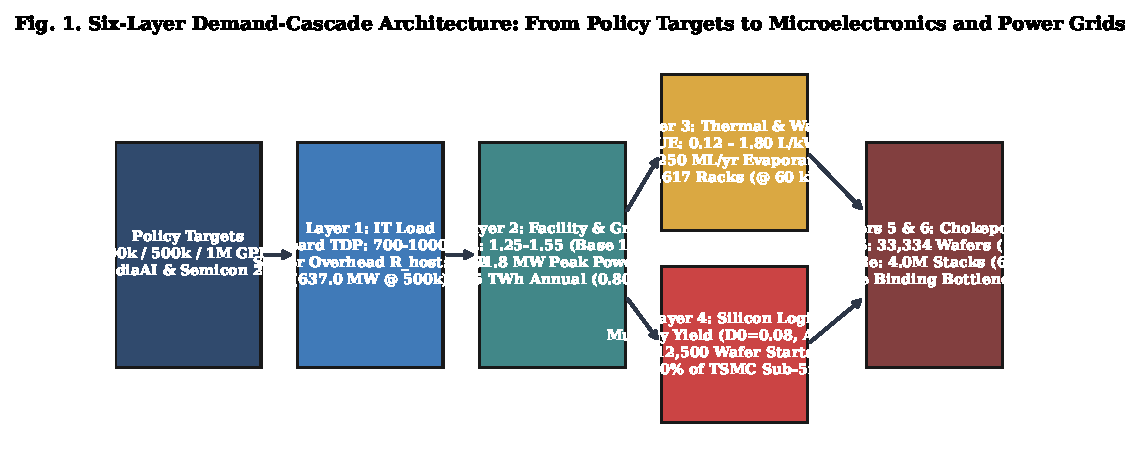
\includegraphics[width=0.94\textwidth]{figures/fig1_demand_cascade_architecture.pdf}\vspace{-2mm}
\caption{Six-layer Demand-Cascade Model with 500{,}000-GPU baseline outputs. Inputs from \cite{nvidia2024h100,lbnl2024datacenter,sbicap2025datacentre,iea2024aienergy,trendforce2026foundry,tsmc2025annual}; values computed by model v2.0.}
\label{fig:cascade}
\end{figure*}

\section{Demand-Cascade Model Formulation}

The DCM maps an accelerator target $N$ (GPUs) through six deterministic computational layers grounded in verified empirical parameters (Fig.~\ref{fig:cascade}).

\subsection{Layer~1: IT Electrical Load}

Active IT power uses reference TDP $P_{\text{gpu}} = 700$~W (NVIDIA H100~SXM5 \cite{nvidia2024h100}) and server chassis overhead $R_{\text{host}} = 1.82$:
\begin{equation}
  P_{\text{IT}} = \frac{N \cdot P_{\text{gpu}} \cdot R_{\text{host}}}{10^{6}} \quad [\text{MW}]
  \label{eq:it_load}
\end{equation}

\subsection{Layer~2: Facility Power and Annual Energy}

Facility draw uses tropical baseline $\text{PUE} = 1.40$; annual energy uses 80\% utilisation over 8{,}760~hr:
\begin{equation}
  P_{\text{facility}} = P_{\text{IT}} \cdot \text{PUE} \quad [\text{MW}]
  \label{eq:facility}
\end{equation}
\begin{equation}
  E_{\text{annual}} = \frac{P_{\text{facility}} \cdot 8{,}760 \cdot U}{10^{6}} \quad [\text{TWh}]
  \label{eq:energy}
\end{equation}
GHG emissions apply the CEA grid factor $\text{EF}_{\text{grid}} = 0.716$~tCO$_2$/MWh \cite{cea2026transmission}:
\begin{equation}
  \text{GHG} = E_{\text{annual}} \cdot \text{EF}_{\text{grid}} \quad [\text{Mt CO}_2/\text{yr}]
  \label{eq:ghg}
\end{equation}

\subsection{Layer~3: Cooling Water and Rack Footprint}

Annual evaporative water withdrawal uses $I_{\text{water}} = 1.80$~L/kWh for tropical air cooling \cite{iea2024aienergy}:
\begin{equation}
  W_{\text{annual}} = \frac{E_{\text{annual}} \cdot 10^{9} \cdot I_{\text{water}}}{10^{6}} \quad [\text{ML}]
  \label{eq:water}
\end{equation}
Physical rack count at $D_{\text{rack}} = 60$~kW/rack:
\begin{equation}
  N_{\text{rack}} = \left\lceil \frac{P_{\text{IT}} \times 10^{3}}{D_{\text{rack}}} \right\rceil
  \label{eq:racks}
\end{equation}

\subsection{Layer~4: Semiconductor Wafer Starts}

Gross dies per 300~mm wafer ($r=150$~mm, $A_{\text{die}}=814$~mm$^2$, GH100 reticle):
\begin{equation}
  N_{\text{gross}} = \left\lfloor \frac{\pi r^{2}}{A_{\text{die}}} - \frac{2\pi r}{\sqrt{2A_{\text{die}}}} \right\rfloor = 63
  \label{eq:gross}
\end{equation}
Murphy defect-density yield ($D_0 = 0.08$~cm$^{-2}$, bounds $[0.06, 0.12]$):
\begin{equation}
  Y_{\text{Murphy}} = \left( \frac{1 - e^{-D_0 A_{\text{die}}}}{D_0 A_{\text{die}}} \right)^2 \approx 0.540
  \label{eq:murphy}
\end{equation}
With industrial binning ($Y = 0.65$, $N_{\text{good}} = 40$ dies/wafer), required wafer starts:
\begin{equation}
  W_{\text{starts}} = \left\lceil \frac{N}{N_{\text{good}}} \right\rceil
  \label{eq:wafers}
\end{equation}

\subsection{Layers~5--6: CoWoS Packaging and HBM}

Each GPU requires one CoWoS 2.5D interposer (15~packages/300~mm wafer, $C_{\text{CoWoS}}=15$):
\begin{equation}
  W_{\text{CoWoS}} = \left\lceil \frac{N}{C_{\text{CoWoS}}} \right\rceil
  \label{eq:cowos}
\end{equation}
Global CoWoS capacity: $\approx$450{,}000~wafers/yr; TSMC controls $\approx$90\% (HHI~=~8{,}100) \cite{trendforce2026foundry}. HBM3e stacks per GPU ($N_{\text{stacks}} = 6$, H100/H200 class; 8 for B200):
\begin{equation}
  N_{\text{HBM}} = N \cdot N_{\text{stacks}}
  \label{eq:hbm}
\end{equation}
Global HBM3e output is $\approx$60M stacks/yr; India has zero domestic production.

\section{Empirical Results and Cross-Pillar Analysis}

\subsection{Scenario Simulation Results}

Table~\ref{tab:scenarios} presents DCM output across three deployment scenarios and three sensitivity variants. Low variant: $P_{\text{gpu}}=700$~W, PUE~=~1.25; Base variant: $P_{\text{gpu}}=700$~W, PUE~=~1.40; High variant: $P_{\text{gpu}}=1{,}200$~W, PUE~=~1.55. In the baseline 500{,}000-GPU scenario, active IT load reaches 637.0~MW and peak facility power escalates to \textbf{891.8~MW}---equivalent to \textbf{56.62\%} of India's mid-2026 operational colocation capacity of 1{,}575~MW \cite{sbicap2025datacentre,cbre2026indiadc}. Annual electricity consumption totals \textbf{6.25~TWh/year}, generating 4.47~Mt~CO$_2$, and evaporative water demand reaches \textbf{11{,}249.5~ML/year}. The 1M-GPU high scenario generates 3{,}255~MW, exceeding India's current capacity by 2.07$\times$. The tornado profile in Fig.~\ref{fig:sensitivity} shows that GPU board power ($+42.9\%$ at 1{,}000~W) causes the largest deviation in peak power, followed by host overhead ($-12.1\%$ to $+15.4\%$) and PUE ($\pm10.7\%$), while cooling WUE drives water demand ($-88.9\%$ to $+38.9\%$).

\begin{table*}[t]
\centering
\caption{Demand-Cascade Model Simulation Results Across GPU Deployment Scenarios (Model v2.0) [Sources: \cite{sbicap2025datacentre,tsmc2025annual,trendforce2026foundry,lbnl2024datacenter}]}
\label{tab:scenarios}
\footnotesize
\begin{tabular*}{\textwidth}{@{\extracolsep{\fill}}llrrrrrrrrr@{}}
\toprule
\textbf{Scenario} & \textbf{Var.} & \textbf{IT~MW} & \textbf{Fac.~MW} & \textbf{TWh/yr} & \textbf{Water~ML} & \textbf{Wafers} & \textbf{TSMC\%} & \textbf{CoWoS} & \textbf{CoWoS\%} & \textbf{Colo\%} \\
\midrule
\multirow{3}{*}{200k GPUs}
 & Low  & 224.0 & 280.0 & 1.59 & 318.9 & 4{,}256 & 0.55\% & 11{,}112 & 2.47\% & 17.78\% \\
 & Base & 254.8 & 356.7 & 2.50 & 4{,}499.8 & 5{,}000 & 0.64\% & 13{,}334 & 2.96\% & 22.65\% \\
 & High & 420.0 & 651.0 & 5.13 & 12{,}831.2 & 6{,}667 & 0.85\% & 16{,}667 & 3.70\% & 41.33\% \\
\midrule
\multirow{3}{*}{500k GPUs}
 & Low  & 560.0 & 700.0 & 3.99 & 797.2 & 10{,}639 & 1.36\% & 27{,}778 & 6.17\% & 44.44\% \\
 & Base & 637.0 & \textbf{891.8} & \textbf{6.25} & \textbf{11{,}249.5} & 12{,}500 & 1.60\% & 33{,}334 & \textbf{7.41\%} & \textbf{56.62\%} \\
 & High & 1{,}050.0 & 1{,}627.5 & 12.83 & 32{,}078.0 & 16{,}667 & 2.14\% & 41{,}667 & 9.26\% & 103.33\% \\
\midrule
\multirow{3}{*}{1M GPUs}
 & Low  & 1{,}120.0 & 1{,}400.0 & 7.97 & 1{,}594.3 & 21{,}277 & 2.73\% & 55{,}556 & 12.35\% & 88.89\% \\
 & Base & 1{,}274.0 & 1{,}783.6 & 12.50 & 22{,}499.0 & 25{,}000 & 3.21\% & 66{,}667 & 14.81\% & 113.24\% \\
 & High & 2{,}100.0 & 3{,}255.0 & 25.66 & 64{,}156.1 & 33{,}334 & 4.27\% & 83{,}334 & 18.52\% & 206.67\% \\
\bottomrule
\end{tabular*}
\end{table*}

\subsection{Monte Carlo Uncertainty}

To see how the base case moves when inputs vary together, we ran 1{,}000 draws (seed 42) at 500k GPUs. Each draw samples independently and uniformly: GPU power 650--850~W, host ratio 1.65--2.05, PUE 1.25--1.55, utilisation 0.70--0.90, WUE 0.30--2.20~L/kWh, $D_0$ 0.06--0.11~cm$^{-2}$, and 14, 15 or 16 packages per interposer wafer. Table~\ref{tab:mc} gives the percentiles. The median facility power (963~MW) sits above the base case because the sampled GPU power is centred on 750~W, not 700~W. Across the central 80\% of draws, facility power equals 51--71\% of operational colocation capacity, CoWoS demand is 6.9--7.9\% of global capacity, and wafer demand is only 1.4--1.9\% of TSMC output, so the chokepoint ordering holds throughout.

\begin{table}[t]
\centering
\caption{Monte Carlo Percentiles at 500k GPUs (1{,}000 Draws, Model v2.0)}
\label{tab:mc}
\footnotesize
\begin{tabular*}{\columnwidth}{@{\extracolsep{\fill}}lrrr@{}}
\toprule
\textbf{Output} & \textbf{P10} & \textbf{P50} & \textbf{P90} \\
\midrule
Peak facility power (MW) & 809.2 & 963.1 & 1{,}114.4 \\
Annual energy (TWh) & 5.69 & 6.79 & 8.24 \\
Cooling water (ML/yr) & 3{,}515.5 & 8{,}186.0 & 13{,}570.9 \\
Logic wafer starts & 11{,}112 & 12{,}821 & 14{,}706 \\
CoWoS interposer wafers & 31{,}250 & 33{,}334 & 35{,}715 \\
\bottomrule
\end{tabular*}
\end{table}

\subsection{Finding~1: Refuting the Silicon Wafer Hypothesis}

The common assumption in sovereign-compute policy is that domestic wafer fabrication is the main bottleneck. The model does not support this. Deploying 500{,}000 accelerators needs only \textbf{12{,}500} 300~mm wafer starts, or \textbf{1.60\%} of TSMC's roughly 780{,}000 sub-5\,nm wafers per year \cite{tsmc2025annual}, a volume that capacity-reservation contracts can cover. A domestic leading-edge fab, by contrast, takes years to qualify and only pays off at high wafer volumes, so building one to serve 1.60\% of demand would misdirect capital.

\subsection{Finding~2: Structural Chokepoint Inversion}

Wafer demand is small, so the binding limits lie elsewhere (Table~\ref{tab:chokepoints}, Fig.~\ref{fig:inversion}). \textbf{CoWoS packaging:} 33{,}334 interposer wafers take \textbf{7.41\%} of global capacity (HHI~=~8{,}100), which is \textbf{4.6$\times$} the load placed on front-end wafers. \textbf{HBM3e:} 3.0M stacks take \textbf{5.00\%} of annual output from a three-supplier market with no Indian production. \textbf{Metropolitan power:} delivering 891.8~MW to Mumbai, which already holds 52.4\% of national capacity, needs about 18 substations of 50~MW each under CEA planning norms \cite{cea2026transmission}, and high-voltage equipment lead times run to 36--48 months.

\begin{figure}[t]
\centering
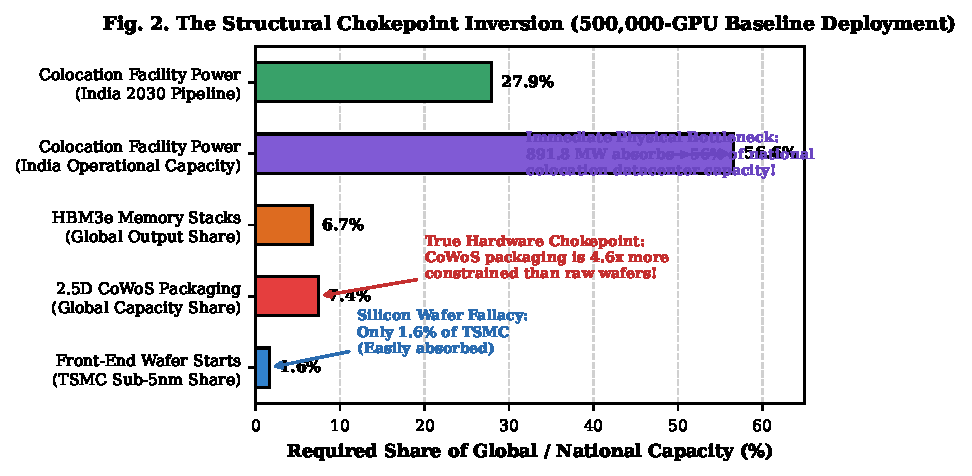
\includegraphics[width=\columnwidth]{figures/fig2_structural_chokepoint_inversion.pdf}\vspace{-2mm}
\caption{Structural chokepoint inversion at the 500{,}000-GPU baseline: packaging (7.41\%) and colocation power (56.62\%) far outstrip logic wafer demand (1.60\%). Denominators from \cite{tsmc2025annual,trendforce2026foundry,counterpoint2025hbm,sbicap2025datacentre}.}
\label{fig:inversion}
\end{figure}

\begin{table}[t]
\centering
\caption{Structural Chokepoint Hierarchy (500k GPU Baseline) [Sources: \cite{akimitsu2026chokepoints,tsmc2025annual,trendforce2026foundry,cea2026transmission,fsr2026powergrid}]}
\label{tab:chokepoints}
\footnotesize
\begin{tabular*}{\columnwidth}{@{\extracolsep{\fill}}lrrrr@{}}
\toprule
\textbf{Infrastructure Layer} & \textbf{HHI} & \textbf{India\%} & \textbf{500k\%} & \textbf{Lead Time} \\
\midrule
EUV Lithography (ASML) & 10{,}000 & 0\% & Upstream & 24--36~mos \\
Sub-5nm Logic (TSMC) & N/A & 0\% & \textbf{1.60\%} & 14--18~wks \\
CoWoS Packaging (TSMC) & 8{,}100 & 0\% & \textbf{7.41\%} & 20--28~wks \\
HBM3e (SK/Samsung/Micron) & 4{,}718 & 0\% & \textbf{5.00\%} & 16--24~wks \\
Colocation Power (India) & N/A & 100\% & \textbf{56.62\%} & 36--48~mos \\
Municipal Water Rights & N/A & 100\% & 11{,}250~ML & Seasonal \\
\bottomrule
\end{tabular*}
\end{table}

\subsection{Finding~3: Tropical Cooling Penalty and Water Vulnerability}

Table~\ref{tab:cooling} compares four cooling options at the 500k-GPU scale. Evaporative towers in sustained summer heat ($>$42\textdegree C) push facility PUE to 1.65; at the annual PUE of 1.45 they evaporate \textbf{11{,}651~ML/yr}. Assuming an urban supply norm of 135~L per person per day (our planning assumption), this equals the domestic demand of roughly 236{,}000 residents. High ambient temperature also shortens hardware life, because thermal fatigue in 2.5D interposer joints and dielectric ageing in HBM through-silicon vias are both temperature-accelerated \cite{ieeetcpmt2026cooling}. Direct-to-chip (D2C) liquid cooling with dry coolers avoids both problems: annual water use falls by \textbf{94.6\%} (to 632~ML/yr) and facility load drops by \textbf{172~MW} (annual PUE 1.18).

\begin{table}[t]
\centering
\caption{Cooling Technology Trade-Off Matrix Under Tropical Climates (500k GPUs) [Sources: \cite{ieeetcpmt2026cooling,fsr2026powergrid,lbnl2024datacenter}]}
\label{tab:cooling}
\footnotesize
\begin{tabular*}{\columnwidth}{@{\extracolsep{\fill}}p{2.6cm}rrrr@{}}
\toprule
\textbf{Cooling System} & \textbf{Ann.~PUE} & \textbf{Peak~PUE} & \textbf{WUE} & \textbf{Water (ML)} \\
\midrule
Traditional Air (Evap.) & 1.45 & 1.65 & 1.80 & 11{,}651.3 \\
Rear-Door Heat Ex. & 1.35 & 1.45 & 1.00 & 6{,}026.5 \\
Direct-to-Chip (D2C) & \textbf{1.18} & \textbf{1.25} & \textbf{0.12} & \textbf{632.1} \\
Single-Phase Immersion & 1.12 & 1.18 & 0.03 & 150.0 \\
\bottomrule
\end{tabular*}
\end{table}

\subsection{Finding~4: Sovereign Compute Scale and Tariff Structure}

India's shared sovereign pool holds roughly 34{,}000--45{,}000 accelerators, against a policy target of 100{,}000 by end-2026 \cite{eetimes2026aimission}. The 500k-GPU baseline analysed here is therefore 11 to 15 times the present pool, and even the 200k scenario is 4 to 6 times larger. Hardware of this class (H100/B200) depends on US Export Administration Regulations and bilateral channels such as iCET \cite{whitehouse2023icet}. On price, the IndiaAI Mission charges Rs.~65 per GPU-hour ($\approx$\$0.78) against market rates of \$2.00--2.80 per hour \cite{sbicap2025datacentre}, a subsidy of 61--72\%. That subsidy rests on stable hardware leasing costs and uninterrupted component supply.

\begin{figure}[t]
\centering
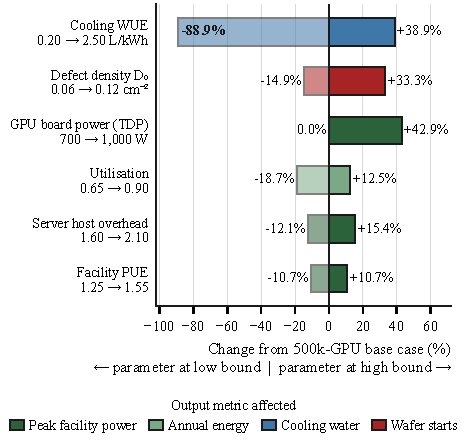
\includegraphics[width=\columnwidth]{figures/fig5_sensitivity_tornado_montecarlo.pdf}\vspace{-2mm}
\caption{One-at-a-time sensitivity of model outputs at 500k GPUs; bounds as in Table~\ref{tab:scenarios} \cite{nvidia2024h100,lbnl2024datacenter,iea2024aienergy}. GPU power dominates peak load; WUE dominates water use.}
\label{fig:sensitivity}
\end{figure}

\section{Strategic Roadmap and Policy Implications}

The cascade findings indicate that industrial interventions should be prioritized by feasibility horizon and strategic autonomy.

\textbf{Tier~1 -- Build Domestically (2026--2028):}
(i)~\textit{Geographic Diversification}: mandate 15--20\% capital rebates for greenfield AI clusters outside Mumbai, targeting Mumbai below 35\% of national capacity by 2028; pre-equip five AI Power Corridors with 400/220~kV infrastructure rated for 5~GW aggregate load.
(ii)~\textit{D2C Cooling Standard}: condition IndiaAI subsidies on PUE $\leq 1.25$ and closed-loop dry heat rejection, saving 11~billion litres/yr at 500k scale.
(iii)~\textit{Fast-Track Substations}: create a 9-month CEA approval window for $\geq$50~MW compute substations; establish an AI Infrastructure Clearance Authority (AICA) under PMO for 90-day composite clearances.
(iv)~\textit{AI Infrastructure Zones (AIZs)}: designate 20 pre-cleared zones across 10 states with pre-built 400~kV substations and 100~Gbps dark fibre.

\textbf{Tier~2 -- Develop Through Partnerships (2028--2031):}
(i)~\textit{Advanced Packaging JVs}: expand Tata Electronics (Morigaon) and Micron Sanand ATMP toward 2.5D silicon interposer via JVs with ASE Group and Ibiden under Semicon~India~2.0, reducing India's 7.41\% CoWoS dependency below 1\% by 2032.
(ii)~\textit{Critical Mineral Refining}: scale CSIR-IMMT hydrometallurgical gallium extraction from NALCO/Hindalco bauxite red mud to an aspirational 50~t/yr of 6N-purity gallium \cite{usgs2025gallium}.
(iii)~\textit{Sovereign Chiplet Consortium}: mobilise 120{,}000 VLSI engineers into a UCIe-standard RISC-V chiplet consortium fabricated at Tata-PSMC Dholera.
(iv)~\textit{Captive Renewable Baseload}: transition AI campuses to Round-the-Clock hybrid solar-wind-BESS power, supplemented by SMRs under the SHANTI Act targeting first nuclear delivery by~2030.

\textbf{Tier~3 -- Manage External Dependencies (2031--2035):}
(i)~\textit{Foundry Reservations}: secure multi-year sovereign wafer allocations at TSMC/Samsung, commercially manageable at 1.60\% of TSMC output.
(ii)~\textit{HBM Supply Treaties}: advance-purchase reservations for HBM4 under the QUAD Semiconductor Supply Chain Initiative.
(iii)~\textit{EAR Contingency Playbook}: formal technology-shock response plans covering various US export restriction scenarios.

\subsection{Investment Architecture}

Table~\ref{tab:investment} sums our planning allocation: about Rs.~95{,}500~crore of public funds and Rs.~2{,}57{,}000~crore expected from private and multilateral partners. These are the authors' proposed envelopes, not budgeted commitments.

\begin{table}[t]
\centering
\caption{Investment Architecture: Three Tiers, Five Pillars (2026--2035) [Sources: \cite{meity2024indiaai,pib2026semicon2,cea2026transmission,usgs2025gallium,denexus2026otcyber}]}
\label{tab:investment}
\footnotesize
\begin{tabular*}{\columnwidth}{@{\extracolsep{\fill}}p{3.0cm}rrp{1.3cm}@{}}
\toprule
\textbf{Intervention Area} & \textbf{Public Rs.~Cr} & \textbf{PPP Rs.~Cr} & \textbf{Lead Agency} \\
\midrule
AIZs \& AICA (P3/P5) & 2{,}500 & 5{,}000 & DPIIT, MeitY \\
Power Corridors + BESS (P2) & 15{,}000 & 65{,}000 & MoP, SECI \\
GPU Cluster Expansion (P1) & 20{,}000 & 80{,}000 & MeitY, IndiaAI \\
Packaging JVs/Gallium (P1) & 10{,}000 & 40{,}000 & ISM, CSIR \\
SMR/Nuclear Baseload (P2) & 25{,}000 & 50{,}000 & DAE, NPCIL \\
Talent \& R\&D (P5) & 15{,}000 & 5{,}000 & MoE, DST \\
Connectivity/Security (P4) & 8{,}000 & 12{,}000 & DoT, NCIIPC \\
\midrule
\textbf{Total} & \textbf{95{,}500} & \textbf{2{,}57{,}000} & \\
\bottomrule
\end{tabular*}
\end{table}

\subsection{Measurable Indicators and Key Performance Metrics}

To operationalise IAIRF~2.0 as an active monitoring instrument, each pillar requires trackable KPIs:
\textbf{P1 (Compute):} Sovereign GPU fleet size; domestic ATMP throughput; VLSI IP registrations; startup compute subsidy uptake.
\textbf{P2 (Energy):} Grid-connection lead time for $\ge$50\,MW compute; captive RTC renewable share; commissioned BESS capacity; average power tariff.
\textbf{P3 (Physical):} Mumbai capacity share ($<$35\% target); D2C liquid-cooled share; PUE; operational AIZs.
\textbf{P4 (Connectivity):} Inter-metro backbone Tbps; DPDPA implementing rules; OT cybersecurity compliance \cite{denexus2026otcyber}; submarine cable landings.
\textbf{P5 (Governance):} AICA 90-day clearance rate; IndiaAI fund disbursement \%; annual AI PhD completions.

\subsection{Scope of Economic Claims}

The DCM quantifies physical requirements rather than macroeconomic returns, so we make no GDP forecast. The cost side is bounded by Table~\ref{tab:investment}: Rs.~3{,}52{,}500~crore in total (public plus PPP). Linking that outlay to output gains would need an input--output model and observed utilisation data from the IndiaAI portal, which we leave to future work.

\section{Limitations and Future Research}

Several assumptions limit the results. First, we fix annual utilisation at $U = 0.80$, which smooths out diurnal inference peaks when substation draw can briefly rise by 20--40\%. Second, foundry defect data are proprietary, so we rely on a published Murphy-model density ($D_0 = 0.08\text{ cm}^{-2}$); across the register range of 0.06--0.12, required wafer starts move by $-14.9\%$ to $+33.3\%$ (Fig.~\ref{fig:sensitivity}). Third, US export rules and bilateral dialogues such as iCET are exogenous to the model and cannot be guaranteed. Fourth, the capacity denominators (TSMC, CoWoS, HBM) are market estimates that will change each year. Future work will feed DCM output into bus-level ACOPF grid simulators for the western and southern grids, using telemetry from the IndiaAI portal, and test whether IAIRF~2.0 transfers to other Global South economies.

\section{Conclusion}

This paper combined the IAIRF~2.0 framework with a six-layer Demand-Cascade Model to test what a 200k to 1M-GPU build-out would demand from India. Three results stand out. Logic wafers are not the constraint: 500k GPUs need 1.60\% of TSMC's sub-5\,nm output, while CoWoS packaging needs 7.41\% of global capacity and colocation power needs 56.62\% of today's operational base. Evaporative cooling in tropical heat is the largest avoidable cost, since direct-to-chip liquid cooling cuts water use by 94.6\% and facility load by 172~MW. Finally, concentration in Mumbai makes the power system fragile. Public spending should therefore favour transmission corridors, packaging partnerships, closed-loop cooling standards and pre-cleared infrastructure zones ahead of a domestic leading-edge fab.

India's strengths are real: VLSI and software talent, multilingual data, early public compute funding, and diplomatic room to manoeuvre. Turning them into sovereignty depends on physical capacity: substations, interposer supply and water-efficient cooling.

\section*{Acknowledgment}
The authors thank Amity University Madhya Pradesh for computing facilities, and the Central Electricity Authority, MeitY and SBI Capital Markets for publicly available reports. The model and figures were scripted in Python (NumPy, Matplotlib) and typeset in \LaTeX. The authors take responsibility for all data interpretation and analysis.

\balance

\bibliographystyle{IEEEtran}
\bibliography{references}

\end{document}
